% 2137 Lab 1 Report
% Created: 2020-01-16, Xingpeng Yi

%==========================================================
%=========== Document Setup  ==============================

% Formatting defined by class file
\documentclass[11pt]{article}

% ---- Document formatting ----
\usepackage[margin=1in]{geometry}	% Narrower margins
\usepackage{booktabs}				% Nice formatting of tables
\usepackage{graphicx}				% Ability to include graphics

%\setlength\parindent{0pt}	% Do not indent first line of paragraphs 
\usepackage[parfill]{parskip}		% Line space b/w paragraphs
%	parfill option prevents last line of pgrph from being fully justified

% Parskip package adds too much space around titles, fix with this
\RequirePackage{titlesec}
\titlespacing\section{0pt}{8pt plus 4pt minus 2pt}{3pt plus 2pt minus 2pt}
\titlespacing\subsection{0pt}{4pt plus 4pt minus 2pt}{-2pt plus 2pt minus 2pt}
\titlespacing\subsubsection{0pt}{2pt plus 4pt minus 2pt}{-6pt plus 2pt minus 2pt}

% ---- Hyperlinks ----
\usepackage[colorlinks=true,urlcolor=blue]{hyperref}	% For URL's. Automatically links internal references.

% ---- Code listings ----
\usepackage{listings} 					% Nice code layout and inclusion
\usepackage[usenames,dvipsnames]{xcolor}	% Colors (needs to be defined before using colors)

% Define custom colors for listings
\definecolor{listinggray}{gray}{0.98}		% Listings background color
\definecolor{rulegray}{gray}{0.7}			% Listings rule/frame color

% Style for Verilog
\lstdefinestyle{Verilog}{
	language=Verilog,					% Verilog
	backgroundcolor=\color{listinggray},	% light gray background
	rulecolor=\color{blue}, 			% blue frame lines
	frame=tb,							% lines above & below
	linewidth=\columnwidth, 			% set line width
	basicstyle=\small\ttfamily,	% basic font style that is used for the code	
	breaklines=true, 					% allow breaking across columns/pages
	tabsize=3,							% set tab size
	commentstyle=\color{gray},	% comments in italic 
	stringstyle=\upshape,				% strings are printed in normal font
	showspaces=false,					% don't underscore spaces
}

% How to use: \Verilog[listing_options]{file}
\newcommand{\Verilog}[2][]{%
	\lstinputlisting[style=Verilog,#1]{#2}
}




%======================================================
%=========== Body  ====================================
\begin{document}

\title{ELC 2137 Lab 1: Git and LateX Intro}
\author{Xingpeng}

\maketitle


\section*{Summary}

This lab introduces two tools suited for programming. One is a control software, Git. It helps you keep track of the modifications people make to the code project and collaborate with others. LaTex is a typesetting language produce professional-looking dcuments. The software helps you focus on working the quality of work because it will help you do the format by coding on it. During this lab, an account of Git is created for each individual student. Intorduces basic operation of uploading files and updating new status of the project to Git. About the LaTex,  lab report was require to be done on the software. Learning functions on the TeXstudio to put chart and figures in your file. 


\section*{Q\&A}
\begin{enumerate}
\item What is your GitHub user name?

Xingpeng-Yi.

\item What LaTeX environment produces a bulleted (non-numbered) list?

Itemize environment
\item  Write  the  equation $y(t) = 1/2 e^t$ using  La-TeX equation formatting.

\$y(t) = 1/2 e\^\ t\$
\item What is the shortcut key for compiling your La-TeX document?

F5



\end{enumerate}
\section*{Results}


\begin{center}
	\begin{tabular}{c|c|c}
		\toprule
		Binary & Hex & Decimal \\
		\midrule
		0000 & 0 & 0 \\
		0010 & 2 & 2 \\
		0100 & 4 & 4 \\
		0110 & 6 & 6 \\
		1000 & 8 & 8 \\
		1010 & A & 10\\
		\bottomrule
	\end{tabular} 
\end{center}

\begin{figure}[ht]\centering
	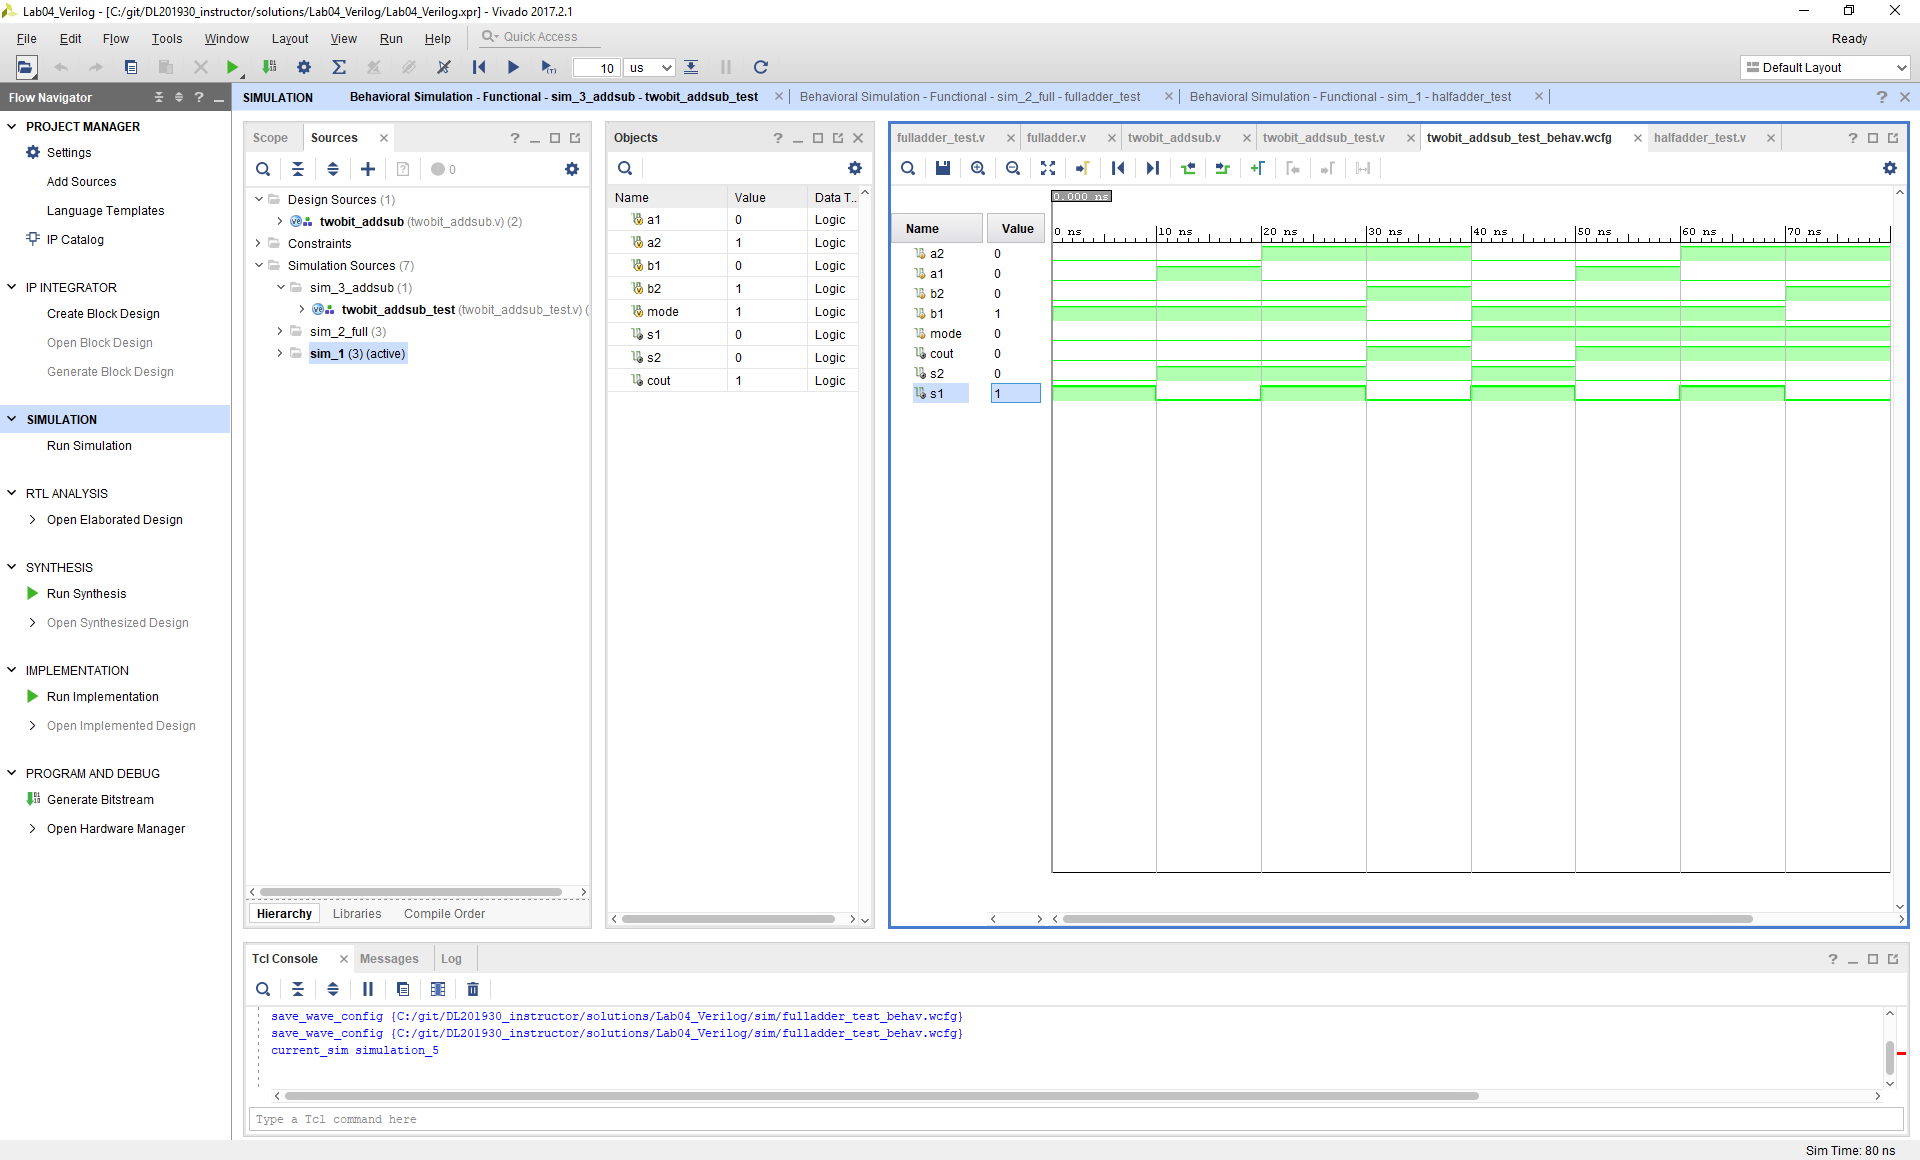
\includegraphics[width=1\textwidth, trim= 19cm 15cm 0.5cm 4cm, clip]{lab1_example_screenshot.PNG}
	\caption{Table and simulation waveform to reproduce.}
	\label{fig:original_logo}
\end{figure}


\section*{Code}

\Verilog{lab1_example_code.sv}

\end{document}
